\documentclass{beamer}
\usepackage{apacite}
\usepackage{graphicx}

\usetheme{Frankfurt}
\graphicspath{{.}}
\setbeamertemplate{caption}[numbered]

% ornate: boadilla frankfurt
% simple: default montpellier singapore szeged34013833


\title{Making sense of spatial demographic data}
\subtitle{}
\author{Chandler Armstrong}
\institute{CERL}
\date{Spring 2019}

\bibliographystyle{apacite}

\begin{document}


\begin{frame}
\titlepage
\end{frame}


\begin{frame}{Agenda}
  \begin{itemize}
  \item Human geography
  \item Human geography and military doctrine
  \item Human geography at CERL
  \item Human geography in RAPTOR
  \item hypothesis testing \& simulation
  \item mapping social vulnerability
    \begin{itemize}
    \item data sources
    \item building the SVI
    \item mapping the SVI to space
    \end{itemize}
  \end{itemize}
\end{frame}


\begin{frame}{Human Geography}
  \begin{definition}{Human Geography}
    Human geography is the branch of geography that deals with the study of people and their communities, cultures, economies, and interactions with the environment by studying their relations with and across space and place.
  \end{definition}
  \begin{definition}{Space}
    Space is the boundless three-dimensional extent in which objects and events have relative position and scale.
  \end{definition}
  Space lacks intrinsic properties; is rarely (never?) an explanatory variable, but patterns in space provide clues to fundamental explanations, and classes of spatial patterns are useful for categorizing other phenomena--e.g. scale free, preferential attachment, concentric zones, multiple nuclei; these spatial patterns contain a lot of information about the machinations of the phenomena they describe.
\end{frame}


\begin{frame}{Human geography and military doctrine}
  \begin{itemize}
  \item Space is universal
  \item Human geography a natural head for organizing broader social science
  \end{itemize}
\end{frame}


\begin{frame}Human geography at CERL}
\begin{itemize}
\item Population simulation \& {\bf interpolation}
\item {\bf Statistical hypothesis testing}
\item {\bf Data integration}
\item GIS
\end{itemize}
\end{frame}


\begin{frame}{Human geography in RAPTOR}
  \begin{itemize}
  \item Disaster impacts and response
  \item Effects of environmental events on conflict
  \item Long-term urban change
  \end{itemize}
\end{frame}


\begin{frame}{Disaster-driven migration}
\end{frame}


\begin{frame}{Data integration}
  \begin{definition}
    indexing of functions or features--e.g. spatial indexing of data-generating functions.
  \end{definition}
  data is often > 90\% of research work; (data integration doesn't magically reduce this)
  \begin{itemize}
  \item reduction
  \item representation
  \item resampling
  \end{itemize}
  identify assumptions of integration, satisfy assumptions during data preprocessing
\end{frame}


\begin{frame}{Data interpolation}
  \begin{itemize}
  \item data spatially indexed and resampled
  \item dasymetric: distribute data between zones based on weights over features:
  \item $z_n = \sum_1^m x_nm \beta_m$
  \item kriging: distribute data between zones based on weights over functions:
  \item $z_n = \sum_1^m z_m \lambda_nm$
  \item regression kriging: kriging with varying mean
  \item $z_n = \sum_1^m (E[z_m]-z_m) \lambda_nm$
  \end{itemize}
\end{frame}


\begin{frame}{Uncertainty}
  \begin{description}
  \item [bayesian] MCMC of posterior
    % normalization constant is intractable
    \begin{description}
    \item [bootstrap] Monte Carlo of empirical data
    \end{description}
  \item [frequentist] standard error
    \begin{description}
    \item [interpolation] uncertainty due to distance from observations
      % \begin{description}
      %   \item [mean] \[K_*^T K^{-1} \bm{y}\]
      %   \item [variance] \[K_{**} - K_*^T K^{-1} K_*\]
      % \end{description}
    \end{description}
  \end{description}
\end{frame}


\begin{frame}{Interpretation}
  \begin{itemize}
  \item data types, assumptions define interpretation
  \item think about interpretation before modeling
    \begin{itemize}
    \item discrete: proportion of people below poverty {\em in an area of space}
    \item continuous: average income {\em in an area of space}
    \end{itemize}
  \item demographic data attached to people, not a continuous random field
  \end{itemize}
\end{frame}


\begin{frame}{Hypothesis testing \& simulation}
  
  \item hypothesis of features; ``x has a significant effect on y''
  \item hypothesis of space; ``cases of x are not randomly distributed across space''
  \begin{itemize}
  \item regression unbiased but inefficient under spatial dependence
  \item spatial modeling a fallback for inability to describe a data generating function
  \item simulate proportions and averages, not people...
  \item estimate demographic indices where no survey data exists
  \item simulate people: where and when, exactly, to place them?
  \end{itemize}
\end{frame}


% if we knew the data generating function sufficiently well, then we could take our observations
% and fit a model to the features that predict the data--this is typical OLS regression
% kriging in general is a solution to our ignorance of how to build this data generating function

\begin{frame}{Data integration}
  \begin{center}
    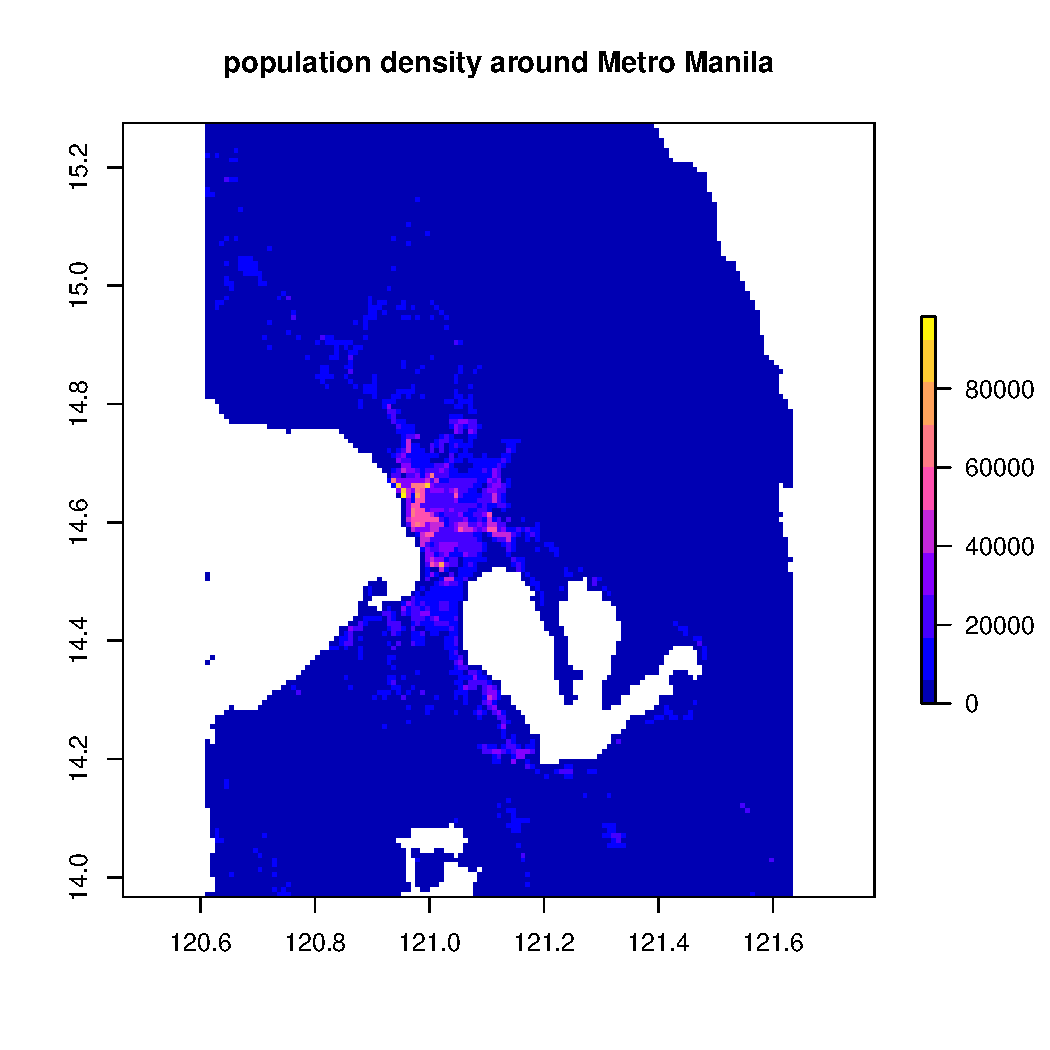
\includegraphics[width=0.4\textheight]{landscan}%
  \end{center}
  \begin{itemize}
  \item people-based (economic, human, \& social capital)
    \begin{itemize}
    \item social networks
    \item education
    \item bank account
    \end{itemize}
  \item place-based (natural, ecological, \& community capital)
    \begin{itemize}
    \item infrastructure (a dam, roads)
    \item natural resources (forest, wetlands)
    \item social services (banks, theatre, retail)
    \end{itemize}
  \end{itemize}
\end{frame}


\begin{frame}{Case: disaster-driven migration}
  \begin{description}
  \item[people-based] propensity to migrate
  \item[place-based] food \& water availability following a disaster
  \end{description}
Grocery stores are a critical source of lifesaving supplies during and after a disaster, however supply chains are often disrupted and unable to deliver the surge of supplies required by the population \cite{palin17}.  Following a disaster, certain types of non-perishable goods may remain sparsely available and out-of-stock for many months \cite{cavallo14}.
\end{frame}


\begin{frame}{Food \& water availability}
  \begin{figure}
  \begin{center}
    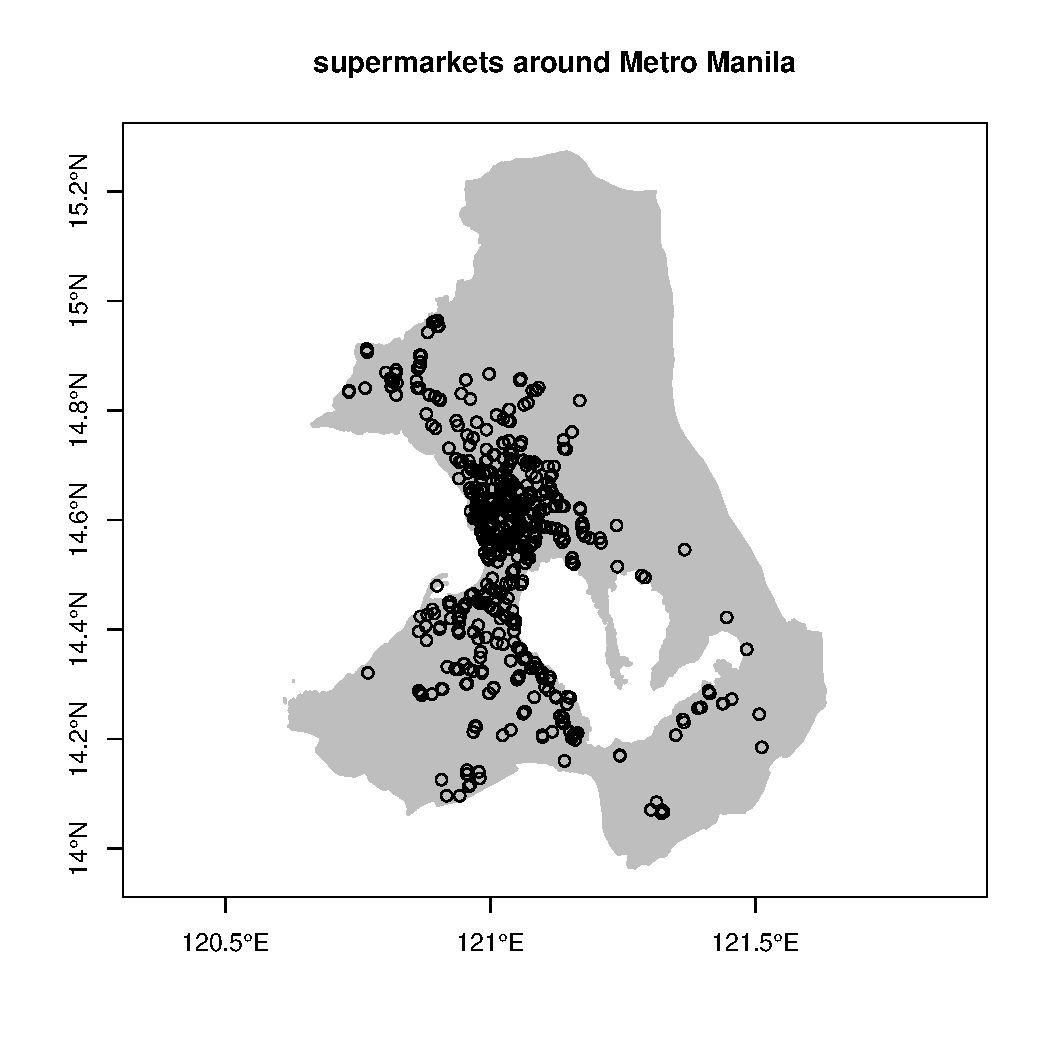
\includegraphics[width=0.3\textwidth]{supermarkets}%
    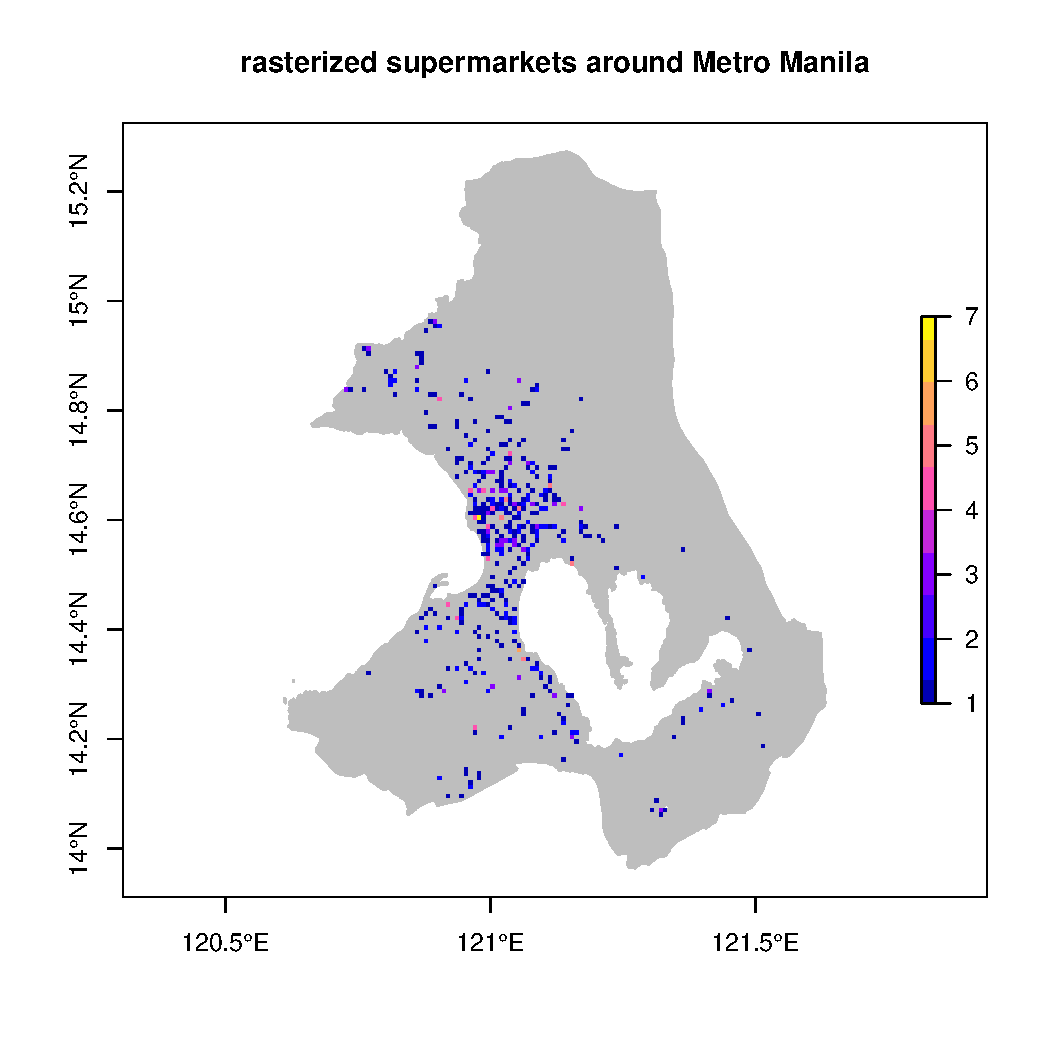
\includegraphics[width=0.3\textwidth]{rSupermarkets}%
    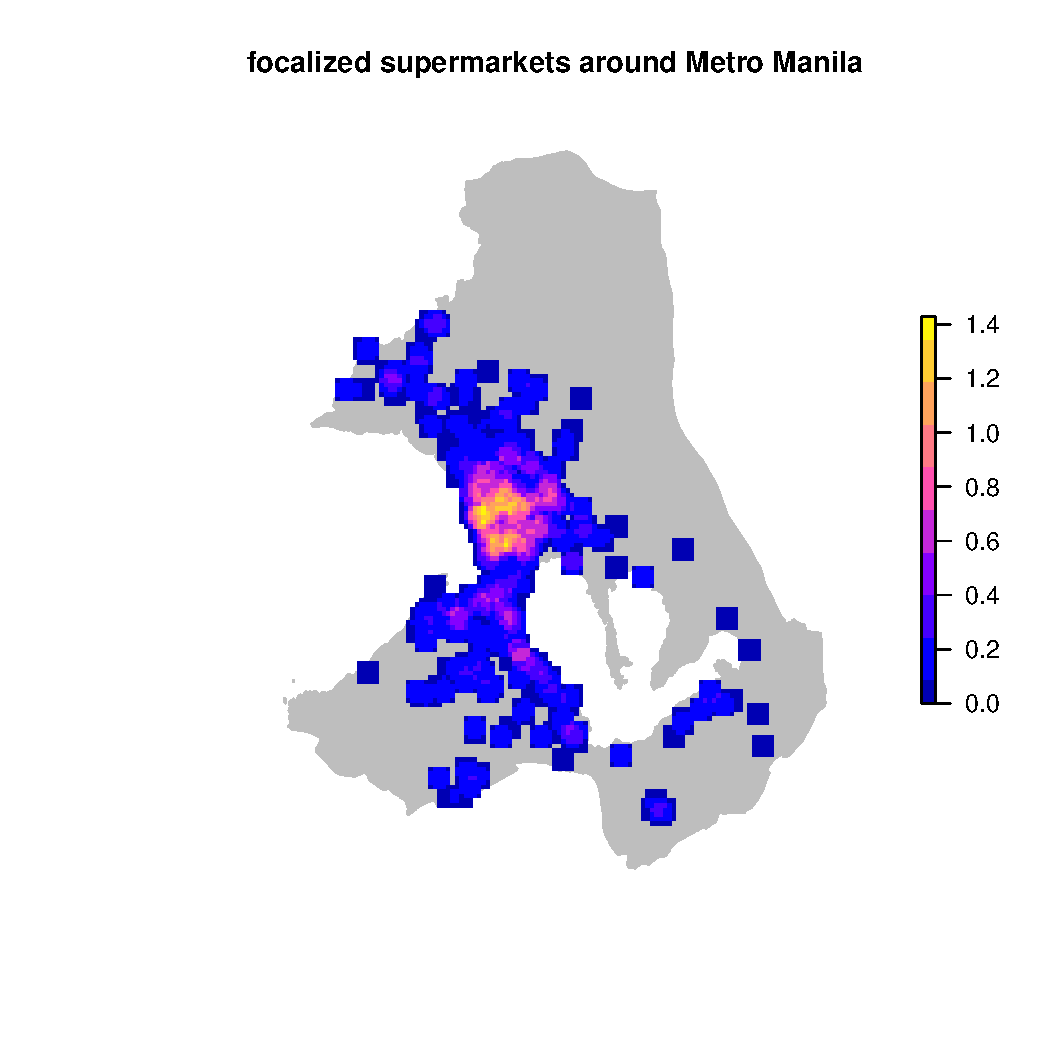
\includegraphics[width=0.3\textwidth]{rSupermarketsFocal}
    % summed into raster cells
  \end{center}
  \caption{\cite{openstreetmap}}
  \end{figure}
  % \begin{itemize}
  % \item supermarkets
  % \end{itemize}
\end{frame}


\begin{frame}{Propensity to migrate}
  \begin{itemize}
  \item past migration
  \item resources to migrate
  \item distance to potential immigration site
  \end{itemize}
  \begin{table}

  \begin{tabular}{l l l}
    \hline
    variable(1=`yes')  & mean(standard deviation) & n missing \\
    \hline
    migration, 5-year  & 0.031(0.03) & 1353467 \\
    migration, 10-year & 0.04(0.038) & 2280714 \\
    native             & 0.98(0.02) & 251850 \\
    % distance to home & & \\
    \hline
   \end{tabular}

  \caption{\cite{ipums}}
  \end{table}

\end{frame}


\begin{frame}{Dasymetric mapping \& population characterization}
  \begin{center}
    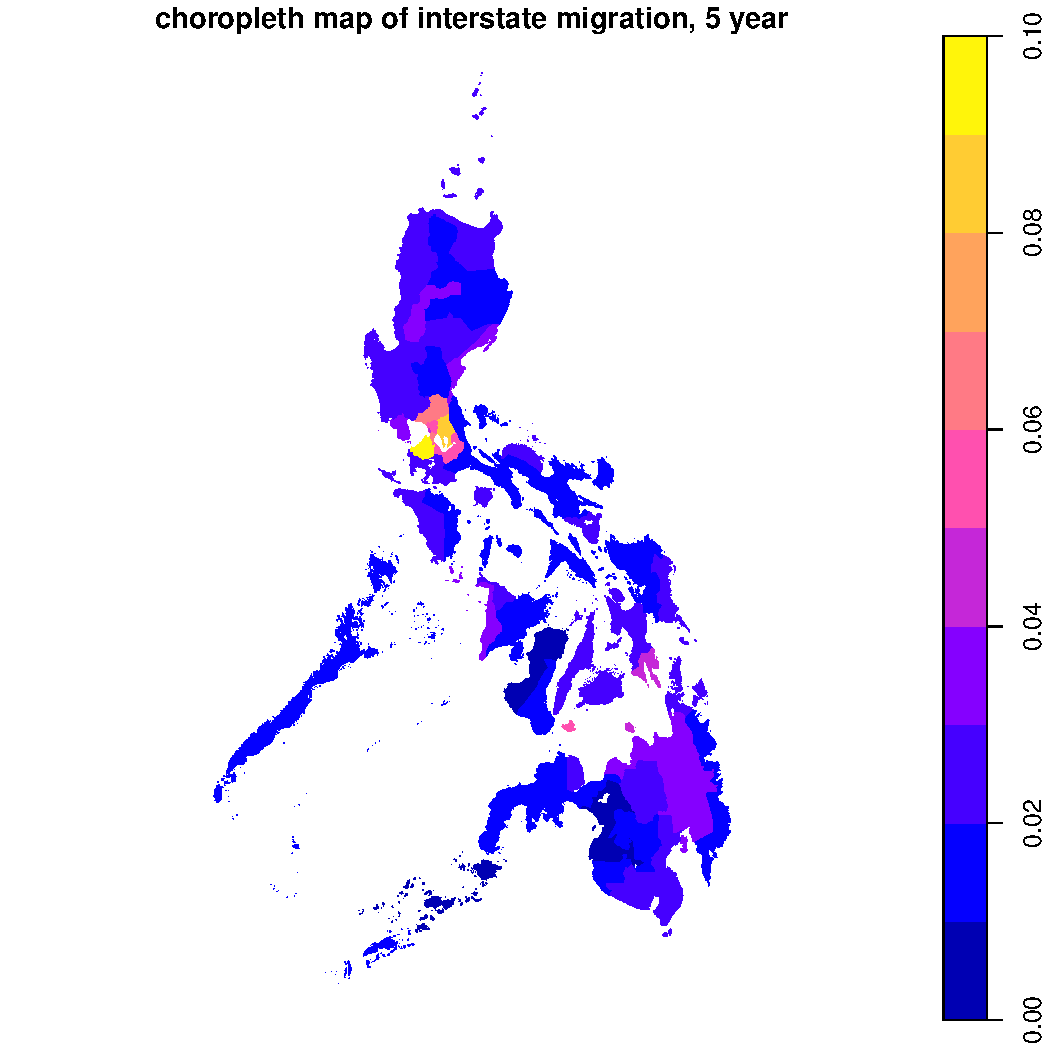
\includegraphics[width=0.3\textwidth]{choropleth}%
    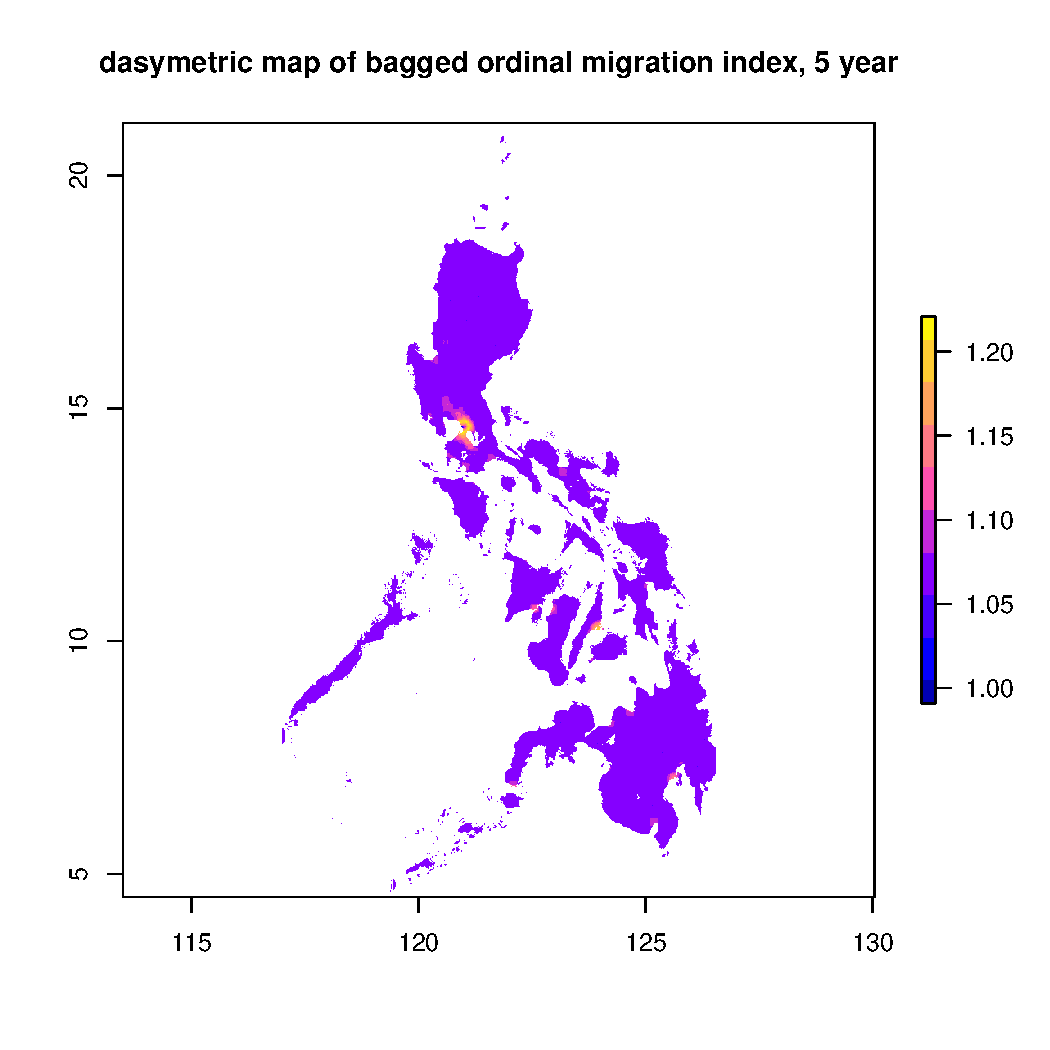
\includegraphics[width=0.3\textwidth]{dasymetric}%
    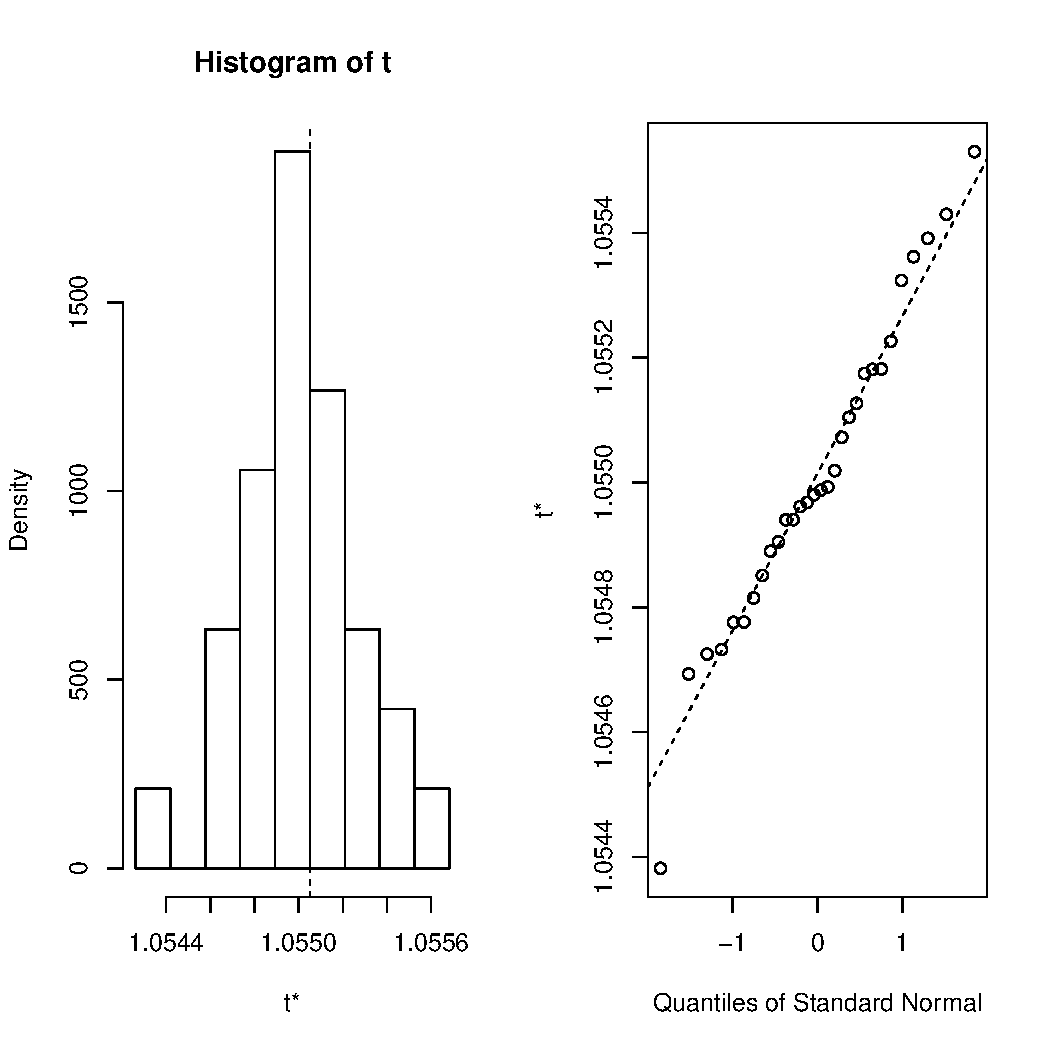
\includegraphics[width=0.3\textwidth]{bagged}
  \end{center}
  % The input population maps are themselves models:
  \begin{itemize}
  \item administrative population data
  \item landcover
  \item roads
  \item points
  \end{itemize}
  % The output of one dasymetric map can be input to another
\end{frame}


\begin{frame}{Linking the wealth of people \& places}
  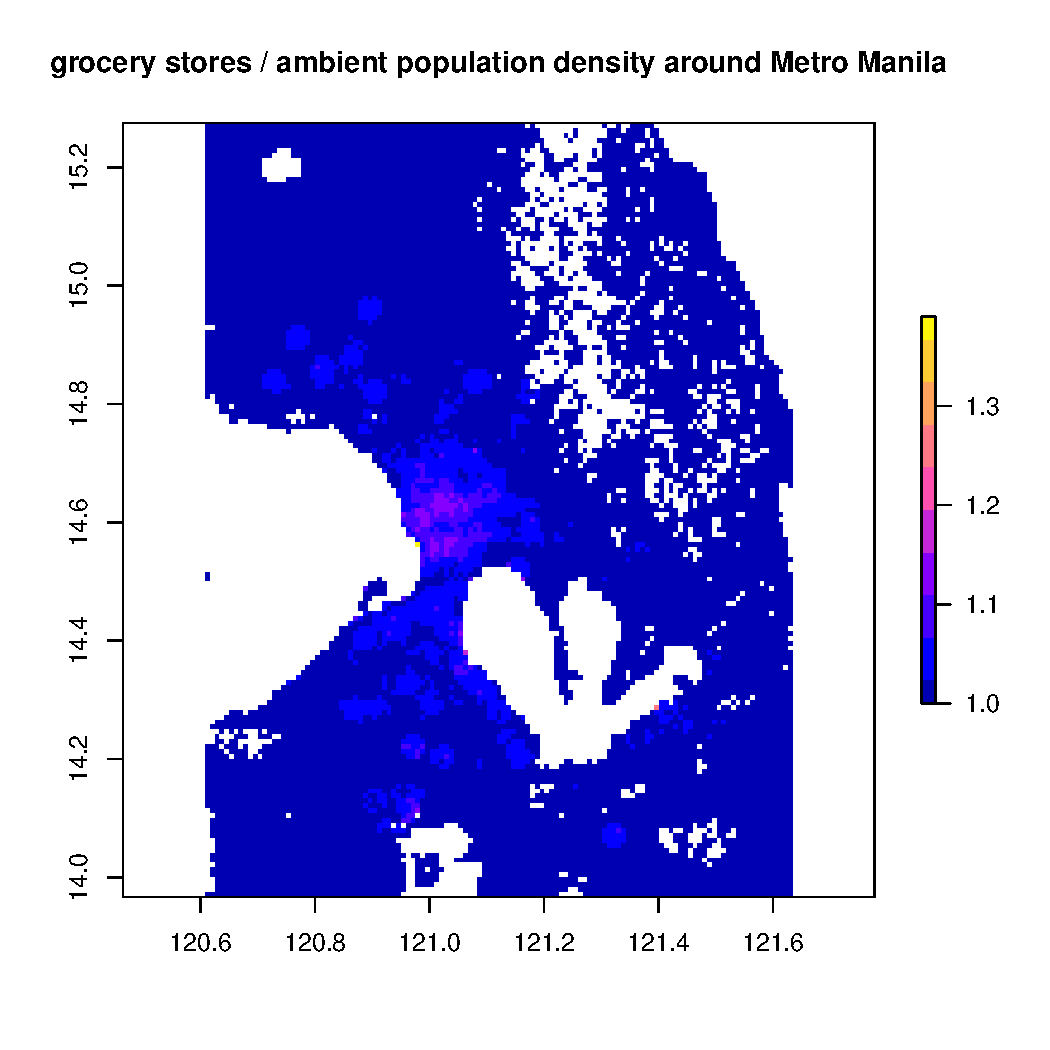
\includegraphics[width=0.3\textwidth]{rSupermarketsFocalNorm}% +
  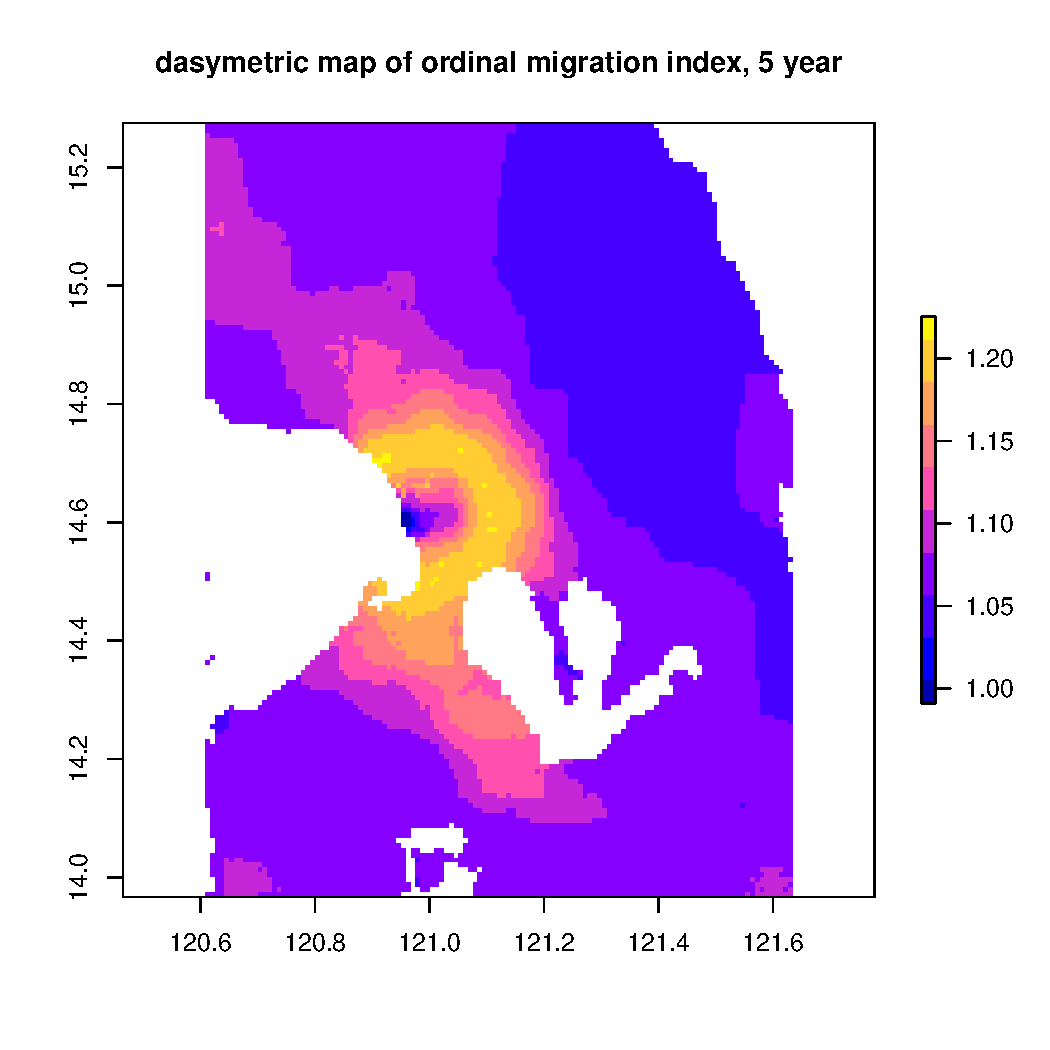
\includegraphics[width=0.3\textwidth]{dasymetricMM}%
  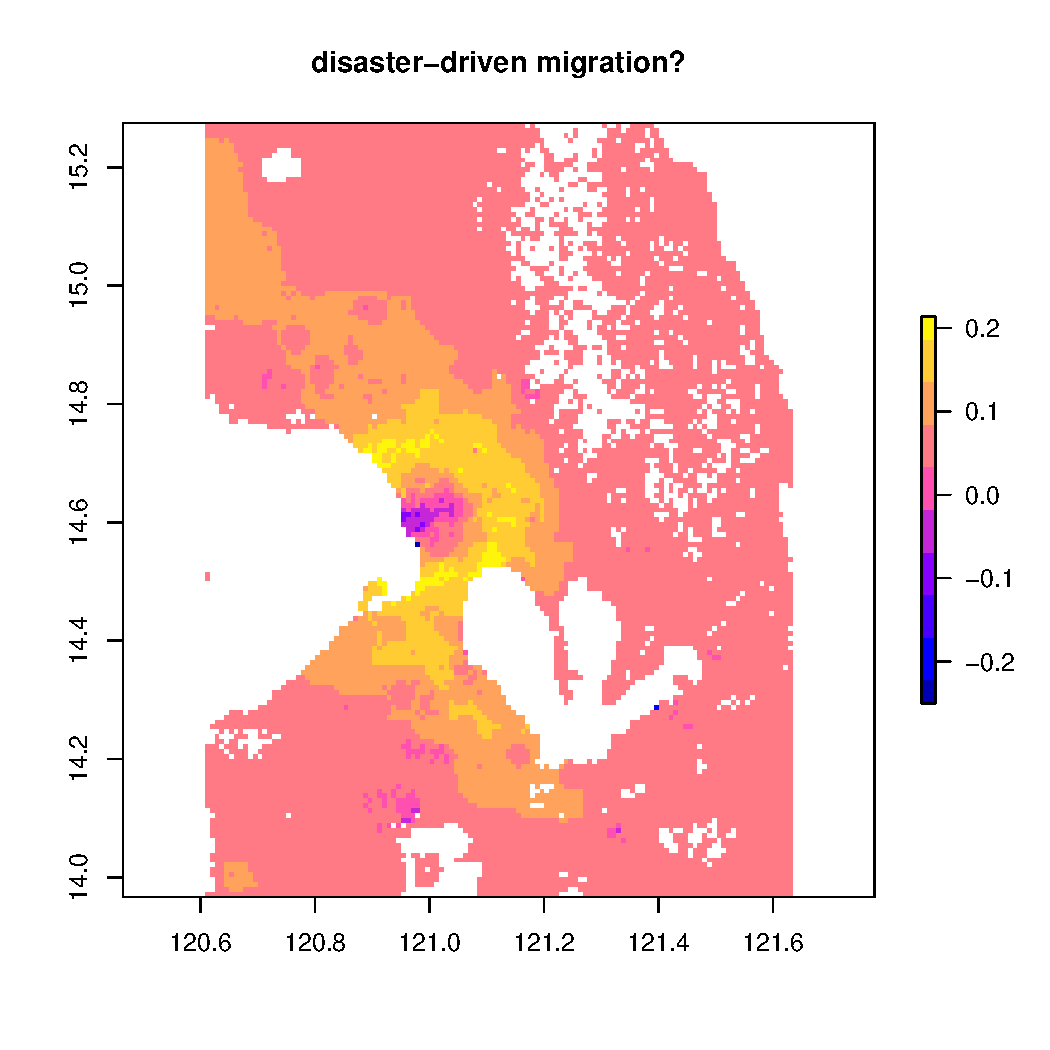
\includegraphics[width=0.3\textwidth]{disaster_driven}
\end{frame}

% \begin{frame}{Research questions}
% \begin{enumerate}
%   \item How do models producing input data influence the output?
%   \item How to include spatial dependence?
%   \item How to incorporate (dirty) point data?
%   \item What does it all mean?
% \end{enumerate}
% \end{frame}


% \begin{frame}{Modelling effects}
%   \begin{center}
%     \includegraphics[height=0.5\textheight]{pop}%
%   \end{center}
%   The input population maps are themselves models:
%   \begin{itemize}
%   \item administrative population data
%   \item landcover
%   \item etc.
%   \end{itemize}
%   How to characterize that relationship?
%   \begin{itemize}
%   \item uncertainty
%   \item multiple equation model
%   \end{itemize}
%   $\Xhat=Z\delta_z+X\delta_x$
%   $\Yhat=\Xhat\Beta+X\Beta$
% \end{frame}


\begin{frame}{Challenges \& Problems}
  \begin{center}
    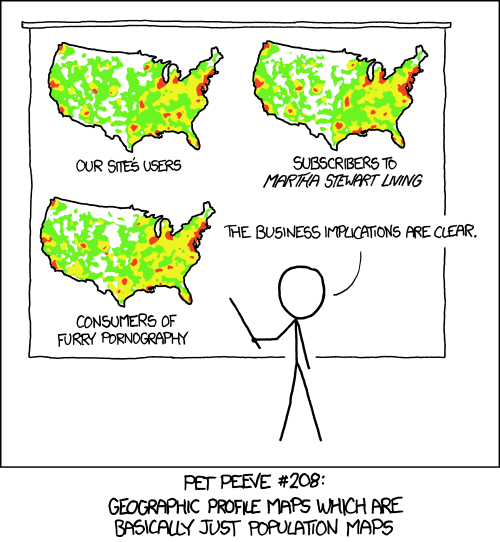
\includegraphics[width=0.4\textheight]{heatmap}
  \end{center}
  \begin{itemize}
  \item Population dominates
  \item Modifiable areal unit problem
  \item Embarrasingly parallel, but high space complexity
  \item Largely deductive, with little to no inductive validation
  \end{itemize}
\end{frame}


% disaster preparedness and mitigation, emergency responses, disaster rehabilitation and reconstruction.
\begin{frame}{Benefits}
  \begin{itemize}
  \item Re-expresses all data into a common format and resolution: easy analysis
  \item Simple to add new data to analysis: resampling \& aggregation
  \item Nonparametric: fast, fewer assumptions, analyze bias, skew, \& uncertainty
  \item Mapped demographics permit geospatial operations: distances, intersections, buffers, etc.
  \item Many applications: disaster preparedness \& mitigation, response, rehabilitation \& reconstruction
  \end{itemize}
\end{frame}
% overlay disaster data or modelled outputs with a characterized population raster and analyze how the affected population can respond through movement or other response strategies.  So, if a certain area of population is affected by water shortages, how far will people travel to obtain what they need?  Do they move to a location with more water, or do they stay and deal with less or lower quality water?  What is the threshold for water availability and quality where people decide to pack up and leave, resulting in disaster driven migration?


\bibliography{disasters}


\begin{frame}{POC}
\begin{description}
  \item[Chandler Armstrong, PI] chandler.m.armstrong@erdc.dren.mil
\end{description}
\end{frame}


\end{document}

%disconcerting conclusion that absent economic motivation ethnic diversity can still lead to violence.  BGD may not generalize well due to relative ethnic homogeneity.  Districts with greater diversity are uncommon and a little diversity in this situation may create tense environments.  It may also be that omitted variables exist correlated with both diversity and violence.  For example access to legitimate political power.

% model indegeneity
% kernel density of fractionalization

% ethnic diversity is really quite rare in BGD, and where it does occur something important may be happening to make these areas, in particular, more violent.  It may not be related to diversity, per se, but to the existence of a particular ethnicity, perhaps an indigenous one.

%%% Local Variables:
%%% mode: latex
%%% TeX-master: t
%%% End:
